\documentclass{article}
\usepackage{graphicx}
\usepackage[italian]{babel}
\usepackage[a4paper, total={500pt, 700pt}]{geometry}
\usepackage{listings}
\usepackage{xcolor}
% Usato per link a referenze
\usepackage{hyperref}
% Necessario per aiutare hyperref a rimandare all'elemento corretto
\usepackage[all]{hypcap}
% Necessario per definire allineamento e larghezza delle colonne nelle tabelle
\usepackage{array}
\newcolumntype{L}[1]{>{\raggedright\let\newline\\\arraybackslash\hspace{0pt}}m{#1}}
\newcolumntype{C}[1]{>{\centering\let\newline\\\arraybackslash\hspace{0pt}}m{#1}}
\newcolumntype{R}[1]{>{\raggedleft\let\newline\\\arraybackslash\hspace{0pt}}m{#1}}

% Per allineamento numerico
\usepackage{siunitx}

\title{Generazione e analisi di eventi di collisione fra particelle}
\author{Lorenzo Redighieri \and Federico Tronchi \and Luca Zoppetti}
\date{30/12/2023}

\definecolor{codegreen}{rgb}{0,0.6,0}
\definecolor{codegray}{rgb}{0.5,0.5,0.5}
\definecolor{codepurple}{rgb}{0.58,0,0.82}
\definecolor{backcolour}{rgb}{0.95,0.95,0.92}

\lstdefinestyle{mystyle}{
    backgroundcolor=\color{backcolour},   
    commentstyle=\color{codegreen},
    keywordstyle=\color{magenta},
    numberstyle=\tiny\color{codegray},
    stringstyle=\color{codepurple},
    identifierstyle=\color{cyan},
    basicstyle=\ttfamily\footnotesize\color{black},
    breakatwhitespace=false,         
    breaklines=true,                 
    captionpos=b,                    
    keepspaces=true,                 
    numbers=left,                    
    numbersep=5pt,                  
    showspaces=false,                
    showstringspaces=false,
    showtabs=false,                  
    tabsize=2
}

\lstset{style=mystyle}

\begin{document}

\maketitle

\section{Introduzione}

Nel corso di tre sessioni di laboratorio sono stati approfonditi i temi del polimorfismo dinamico, del metodo Monte Carlo e dell'analisi dati costruendo un simulatore di eventi di collisione fra particelle con l'ausilio del framework ROOT. Negli eventi di collisione sono state trattate 7 particelle: pioni positivi e negativi ($\pi\pm$), kaoni positivi e negativi ($k\pm$), protoni ($p+$), antiprotoni ($p-$) e particelle K*, che decadono rapidamente in un pione e un kaone di carica opposta. Il programma, il cui scopo è rilevare la presenza della particella K* tramite l'analisi degli effetti del suo decadimento, è diviso in due componenti principali: quella di generazione casuale degli eventi e quella di analisi dati. La prima si occupa di generare e salvare in un file ROOT gli istogrammi con i dati relativi agli eventi di collisione fra le particelle. È implementata nella macro \verb|generate.cpp|, che può essere eseguita in modalità compilata dopo aver compilato nell'ordine anche i file da cui dipende: \verb|ParticleType.cpp|, \verb|ResonanceType.cpp| e \verb|Particle.cpp|. Per eseguirla è necessario indicare due parametri come argomento della funzione \verb|generate()| nel terminale di ROOT: il numero di eventi da generare e il nome del file ROOT in cui salvare gli istogrammi. La seconda parte invece si occupa di eseguire le sottrazioni fra istogrammi e i fit per rilevare il segnale della particella K*. È una macro autonoma implementata interamente nel file \verb|analyse.cpp|. Dopo averla compilata, essa può essere eseguita indicando il nome del file da analizzare come parametro della funzione \verb|analyse()| nel terminale di ROOT. Di seguito vengono trattate le metodologie utilizzate nella scrittura del codice e i risultati del lavoro.

\section{Struttura del codice}
Per rappresentare le particelle sono state implementate tre classi: \verb|ParticleType|, \verb|ResonanceType| e \verb|Particle|.

\verb|ParticleType| contiene le informazioni basilari di una particella: nome, massa e carica, rappresentate da membri privati costanti. Come metodi pubblici sono presenti un costruttore parametrico, un distruttore virtuale, i \textit{getters} dei membri privati (di cui uno virtuale) e la funzione virtuale \verb|print| che stampa i valori di questi ultimi. Le funzioni virtuali sono poi reimplementate nella classe figlia \verb|ResonanceType|, utilizzata per rappresentare una particella instabile, che eredita \verb|ParticleType| con l'aggiunta della larghezza di risonanza, anch'essa membro privato costante. Il \textit{getter} virtuale precedentemente citato è implementato per restituire la larghezza di risonanza.

Queste due classi definiscono le proprietà generiche che caratterizzano una tipologia di particelle, tuttavia, per rappresentare una particolare particella, occorre aggiungervi le informazioni cinematiche, che sono gestite nella classe \verb|Particle|. Essa possiede come membri privati un vettore statico di puntatori (per sfruttare il polimorfismo dinamico) a \verb|ParticleType| contenente i tipi di particelle, un \verb|std::optional<int>| in cui è salvato l'indice dell'elemento che rappresenta il tipo della particella (\verb|std::optional| aiuta a gestire i casi in cui viene impostato un indice errato) e una \verb|struct| chiamata \verb|Momentum| per rappresentare la quantità di moto. L'utilizzo di un vettore statico per i tipi di particelle aumenta l'efficienza del programma, poiché altrimenti sarebbe necessario copiare tutte le informazioni comuni alle particelle per ogni istanza di \verb|Particle|.

La classe \verb|Particle| dispone dei seguenti metodi pubblici:
\begin{itemize}
    \item Il costruttore per creare la particella tramite il nome e la quantità di moto.
    \item I \textit{getters} per i membri privati e la massa invariante.
    \item I \textit{setters} per l'indice della particella e la quantità di moto.
    \item Tre metodi statici per contare i tipi di particelle disponibili, aggiungerne di nuovi e stamparli.
    \item Due metodi per il decadimento delle particelle instabili.
    \item Un metodo che stampa tutte le informazioni della particella.
\end{itemize}

\newpage

\section{Generazione degli eventi}

La generazione degli eventi è stata gestita tramite la macro \verb|generate.cpp|.

Le classi base del programma sono costruite per funzionare con qualsiasi particella e con qualsiasi numero di tipologie di particelle, che in questo specifico caso sono 7: pioni positivi e negativi, kaoni positivi e negativi, protoni, antiprotoni e particelle K*. Un evento consiste nella generazione di 100 particelle secondo le proporzioni riportate nella Tabella \ref{tab:particles_table}.

La quantità di moto di ciascuna particella è stata generata attraverso le seguenti distribuzioni: il suo angolo azimutale è stato estratto da una distribuzione uniforme tra 0 e $ 2 \pi $, l'angolo polare da un'altra distribuzione uniforme tra 0 e $ \pi $ e il modulo da una distribuzione esponenziale decrescente con media pari a 1 GeV.

\begin{table}[ht]\label{tab:particles_table}
    \centering
    \begin{tabular}{|c|c|c|c|c|}
    \hline
    Tipo & Massa (GeV/c$^2$) & Carica (e) & Larghezza (GeV/c$^2$) & Percentuale \\
    \hline
    Pione+ & $1.3957\times10^{-1}$ & +1 & 0 & 40 \% \\
    \hline
    Pione- & $1.3957\times10^{-1}$ & -1 & 0 & 40 \% \\
    \hline
    Kaone+ & $4.9367\times10^{-1}$ & +1 & 0 & 10 \% \\
    \hline
    Kaone- & $4.9367\times10^{-1}$ & -1 & 0 & 10 \% \\
    \hline
    Protone+ & $9.3827\times10^{-1}$ & +1 & 0 & 4.5 \% \\
    \hline
    Protone- & $9.3827\times10^{-1}$ & -1 & 0 & 4.5 \% \\
    \hline
    K* & $8.9166\times10^{-1}$ & 0 & $5.0\times10^{-2}$ & 1 \% \\
    \hline
    \end{tabular}
    \caption{Nella tabella sono riportate le proprietà che caratterizzano le tipologie di particelle utilizzate nella simulazione e le proporzioni con le quali sono state generate in ogni evento. L'unità di misura $e$ rappresenta la carica fondamentale, $e = 1.602176634\times10^{-19}C$.}
\end{table}

 \noindent Nell'eventualità in cui venga generata una particella K*, questa è fatta decadere attraverso il metodo \verb|decayToBody()| in un pione e un kaone di carica opposta.
 Le particelle vengono successivamente combinate per creare gli istogrammi di massa invariante utilizzati nella parte di analisi. Vengono considerate le seguenti combinazioni:
\begin{itemize}
    \item tutte le particelle;
    \item particelle di carica discorde;
    \item particelle di carica concorde;
    \item kaoni e pioni di carica discorde;
    \item kaoni e pioni di carica concorde;
    \item kaoni e pioni provenienti dal decadimento della stessa K*.
\end{itemize}

\section{Analisi dati}
I dati raccolti sono stati analizzati attraverso la macro \verb|analyse.cpp|. Le abbondanze di particelle generate (Tab. \ref{tab:occurrences}) risultano compatibili con le percentuali di generazione (Tab. \ref{tab:particles_table}).

Per gli istogrammi degli angoli e della quantità di moto (Fig. \ref{fig:angles_momentum}) sono stati eseguiti dei fit (Tab. \ref{tab:angles_momentum_fits}) per verificare la compatibilità con i dati di partenza della generazione, uniformi per i primi due ed esponenziale per il terzo, che risultano tutti compatibili con quanto atteso. Per ciascun fit è stato riportato il valore $\widetilde{\chi}^2 = \frac{\chi^2}{DOF}$, che costituisce una misura dell'accordo fra i dati e la relazione funzionale ipotizzata. Un'ipotesi associata a un $\widetilde{\chi}^2 \sim 1$ è considerata accettabile.

Il segnale della particella K* è stato estratto prima studiando la distribuzione della massa invariante dei prodotti del decadimento (\textit{Decay products}, Fig. \ref{fig:k_star}), poi attraverso una sottrazione di istogrammi. Questo secondo metodo si basa sul fatto che il decadimento della K* (che genera pioni e kaoni di carica opposta) produce una leggera differenza nella distribuzione di massa invariante fra le particelle di carica discorde e di carica concorde. L'istogramma \textit{Opposite charge - same charge} (Fig. \ref{fig:k_star}) è stato definito come la sottrazione dell'istogramma di massa invariante di particelle aventi stessa carica dall'istogramma di massa invariante di particelle di carica opposta. Attraverso il fit ad una distribuzione gaussiana sono state ricavate massa e larghezza della K*, corrispondenti a media e deviazione standard della gaussiana. Per l'istogramma \textit{Opposite charge - same charge (kaon \& pion)} (Fig. \ref{fig:k_star}) si è proceduto in maniera analoga, sottraendo l'istogramma di massa invariante dei kaoni e pioni con stessa carica dall'istogramma di massa invariante dei kaoni e pioni con carica opposta. Tutti i valori (Tab. \ref{tab:gaussian_fits}) di massa e larghezza ricavati dai fit gaussiani risultano compatibili entro $2\sigma$ con quelli in input alla generazione.

\newpage

\begin{figure}[ht]\label{fig:angles_momentum}
    \centering
    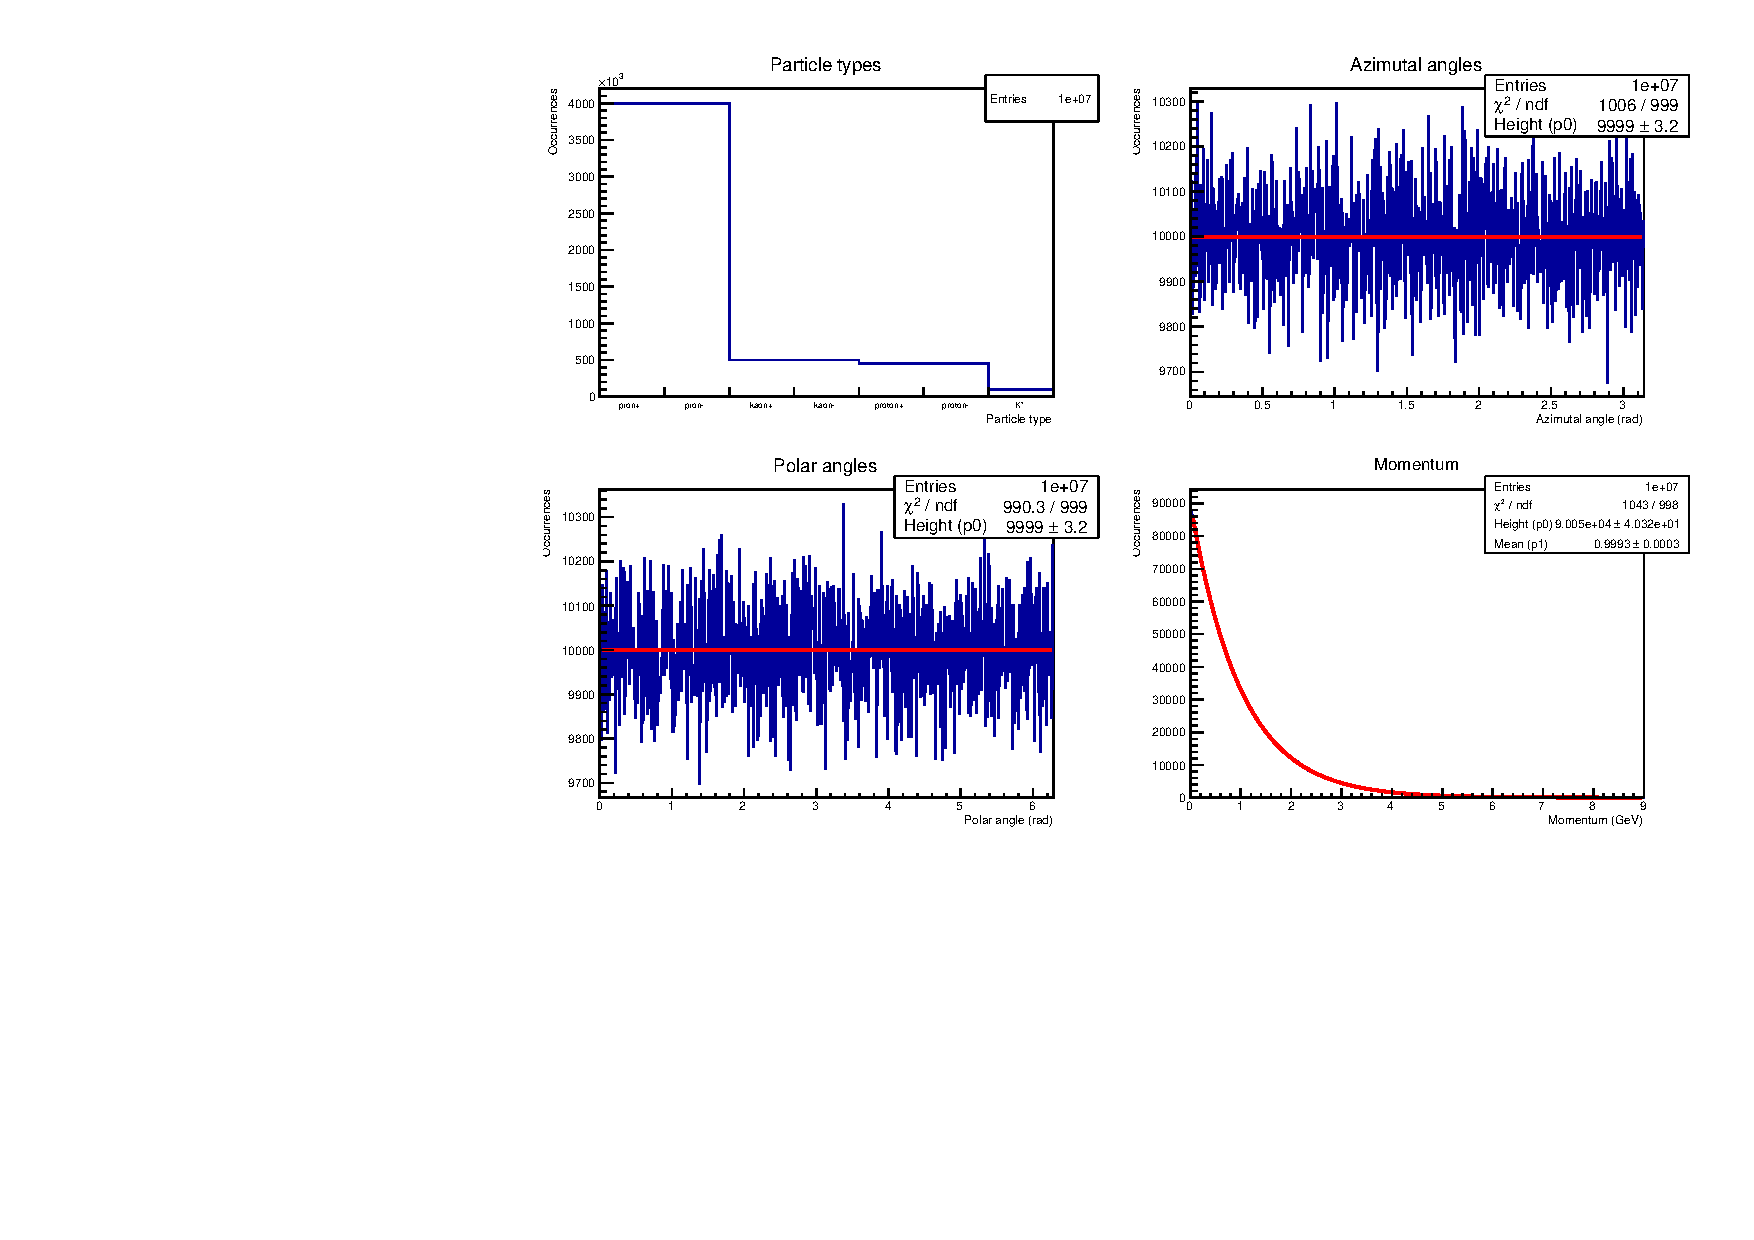
\includegraphics[width=450pt]{images/first_canvas.pdf}
    \caption{La figura contiene gli istogrammi relativi ad abbondanza di distribuzione delle particelle, angolo azimutale, angolo polare e quantità di moto. Ad eccezione del primo sono state definite delle funzioni per il fit degli istogrammi, che sono raffigurate in rosso. I dati raccolti dal primo istogramma sono riportati in Tabella \ref{tab:occurrences}. Nelle legende sono visualizzati i parametri ottenuti dai fit, riportati anche in Tabella \ref{tab:angles_momentum_fits}.}
\end{figure}

\begin{table}[ht]\label{tab:occurrences}
\centering
\begin{tabular} {|c|c|c|}
 \hline
 Specie & Occorrenze Osservate & Occorrenze Attese \\
 \hline
 Pione+ & $(3.999\pm0.002)\times10^{6}$ & $4\times10^{6}$ \\
 \hline
 Pione- & $(4.000\pm0.002)\times10^{6}$ & $4\times10^{6}$ \\
 \hline
 Kaone+ & $(5.008\pm0.007)\times10^{5}$ & $5\times10^{5}$ \\
 \hline
 Kaone- & $(5.002\pm0.007)\times10^{5}$ & $5\times10^{5}$ \\
 \hline
 Protone & $(4.502\pm0.007)\times10^{5}$ & $4.5\times10^{5}$ \\
 \hline
 Antiprotone & $(4.498\pm0.007)\times10^{5}$ & $4.5\times10^{5}$ \\
 \hline
 K* & $(1.003\pm0.003)\times10^{5}$ & $1\times10^{5}$ \\
 \hline
 \end{tabular}
 \caption{Nella tabella sono riportati il tipo delle particelle generate, l'occorrenza di particelle generate per ogni tipo, corrispondente al numero di occorrenze per bin nell'istogramma \textit{Particle types} (Fig. \ref{fig:angles_momentum}), e il numero atteso di particelle generate. Trattandosi di un esperimento di conteggio, l'incertezza sul numero osservato di particelle è stata calcolata come $\sqrt{N}$. Le occorrenze osservate risultano compatibili con quelle attese.}
\end{table}

\begin{table}[ht]\label{tab:angles_momentum_fits}
\centering
\begin{tabular} {|C{0.2\linewidth}|c|c|c|c|c|}
\hline
Distribuzione & Ordinata all'origine & Media (GeV) & $\chi^2$ & DOF & $\widetilde{\chi}^2$ \\
\hline
Fit uniforme, angolo azimutale & $(9.999\pm0.003)\times 10^3$ & ND & 1006 & 999 & 1.01 \\
\hline
Fit uniforme, angolo polare & $(9.999\pm0.003)\times 10^3$ & ND & 990.3 & 999 & 0.99 \\
\hline
Fit esponenziale, modulo dell'impulso & $(9.005\pm0.004)\times10^4$ & $(9.993\pm0.003)\times10^{-1}$ & 1043 & 998 & 1.05 \\
\hline
\end{tabular}
\caption{Nella tabella vengono mostrati i risultati dell'adattamento dei fit agli istogrammi \textit{Azimutal angles, Polar angles, Momentum} (Fig. \ref{fig:angles_momentum}). Ricavando dai fit $\chi^2$ e gradi di libertà (DOF) è stato calcolato $\widetilde{\chi}^2$, confermando che i valori generati sono consistenti con le distribuzioni attese poiché $\widetilde{\chi}^2 \sim 1$. ND indica che il parametro non è disponibile per il fit di riferimento.}
\end{table}

\newpage

\begin{figure}[ht]\label{fig:k_star}
    \centering
    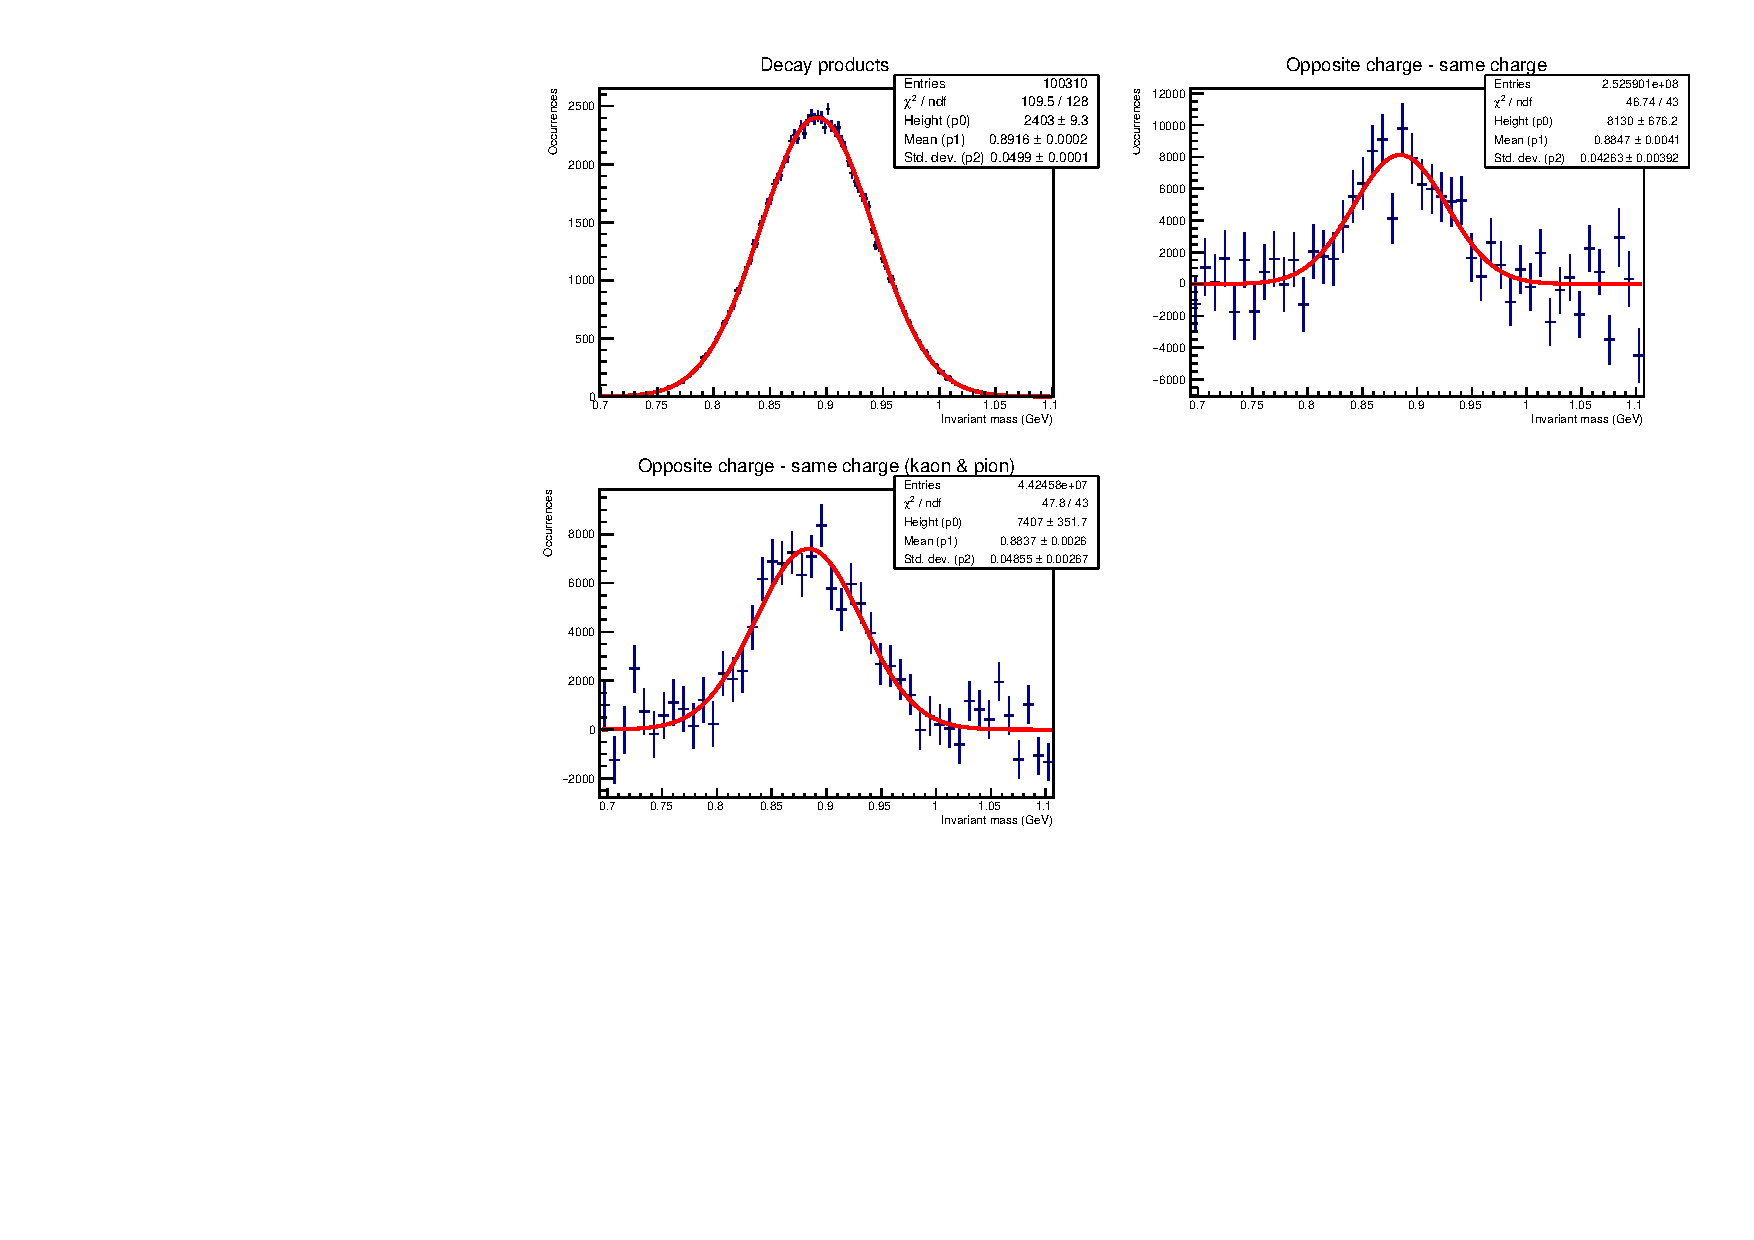
\includegraphics[width=450pt]{images/second_canvas.pdf}
    \caption{In figura vengono mostrati gli istogrammi di massa invariante utilizzati per rilevare il segnale della particella K*. Nel primo sono riportati i valori di massa invariante calcolati unicamente tra i prodotti dei decadimenti. Il secondo e il terzo istogramma sono il risultato di una sottrazione di istogrammi, utilizzata per far emergere il segnale di K* dal fondo. Attraverso un fit, i cui parametri sono visibili nella legenda e in Tabella \ref{tab:gaussian_fits}, è stata verificata la consistenza delle distribuzioni con una gaussiana, rappresentata in rosso.}
\end{figure}

\begin{table}[ht]\label{tab:gaussian_fits}
\centering
\begin{tabular} {|C{0.25\linewidth}|c|c|c|c|}
\hline
Istogramma & Ampiezza & Media (GeV) & Sigma (GeV) & $\widetilde{\chi}^2$ \\
\hline
Massa invariante ottenuta dalle coppie di particelle decadute dalla particella K* & $(2.403\pm0.018) \times 10^3$ & $(8.916\pm0.004) \times 10^{-1}$ & $(4.99\pm0.02) \times 10^{-2}$ &  0.86 \\
\hline
Massa invariante ottenuta da differenza delle combinazioni di carica discorde e concorde & $(8.1\pm1.4)\times10^3$ & $(8.85\pm0.08)\times10^{-1}$ & $(4.3\pm0.8)\times10^{-2}$ & 1.09 \\
\hline
Massa invariante ottenuta da differenza delle combinazioni kaone-pione di carica discorde e concorde & $(7.4\pm0.8)\times10^2$ & $(8.84\pm0.06)\times10^{-1}$ & $(4.9\pm0.6)\times10^{-2}$ & 1.11 \\
\hline
\end{tabular}
\caption{La tabella riporta i risultati dei fit agli istogrammi (Fig. \ref{fig:k_star}) definiti per misurare massa e ampiezza della K*, corrispondenti rispettivamente a media e deviazione standard della distribuzione gaussiana. Le incertezze sono state calcolate come il doppio dell'incertezza fornita dal fit, per cui i risultati sono compatibili entro $2\sigma$ con i dati in input alla generazione. I fit sono accettabili in quanto $\widetilde{\chi}^2\sim 1$.}
\end{table}

\newpage

\section*{Appendice}

\subsection*{ParticleType.hpp}
\lstinputlisting[language=C++]{code/generate/ParticleType.hpp}

\subsection*{ParticleType.cpp}
\lstinputlisting[language=C++]{code/generate/ParticleType.cpp}

\subsection*{ResonanceType.hpp}
\lstinputlisting[language=C++]{code/generate/ResonanceType.hpp}

\subsection*{ResonanceType.cpp}
\lstinputlisting[language=C++]{code/generate/ResonanceType.cpp}

\subsection*{Particle.hpp}
\lstinputlisting[language=C++]{code/generate/Particle.hpp}

\subsection*{Particle.cpp}
\lstinputlisting[language=C++]{code/generate/Particle.cpp}

\subsection*{generate.cpp}
\lstinputlisting[language=C++]{code/generate/generate.cpp}

\subsection*{analyse.cpp}
\lstinputlisting[language=C++]{code/analyse/analyse.cpp}

\end{document}
